\titleframe

\section{Introduction}

\begin{frame}{\insertsectionhead}
  \begin{figure}[H]
    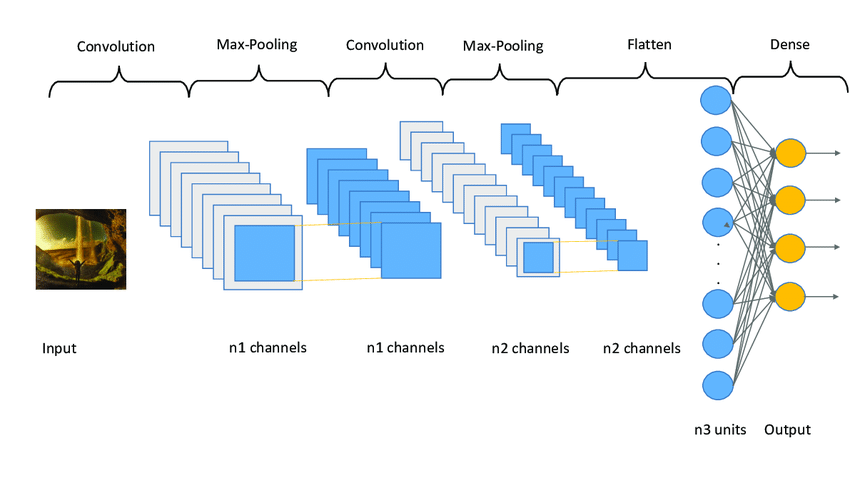
\includegraphics[width=10cm]{Graphics/convolutional.png}
    \caption{Convolutional neural networks\cite{Garcia_2020}.}
  \end{figure}
\end{frame}

\begin{frame}{\insertsectionhead}
  \begin{figure}[H]
    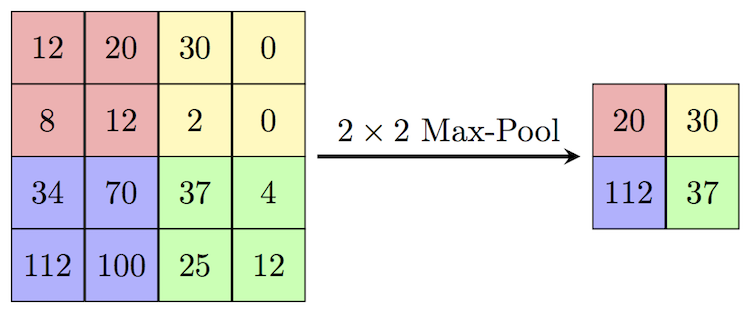
\includegraphics[width=10cm]{Graphics/max_pooling.png}
    \caption{Max pooling layer.}
  \end{figure}
\end{frame}

\begin{frame}{\insertsectionhead}
  \begin{figure}[H]
    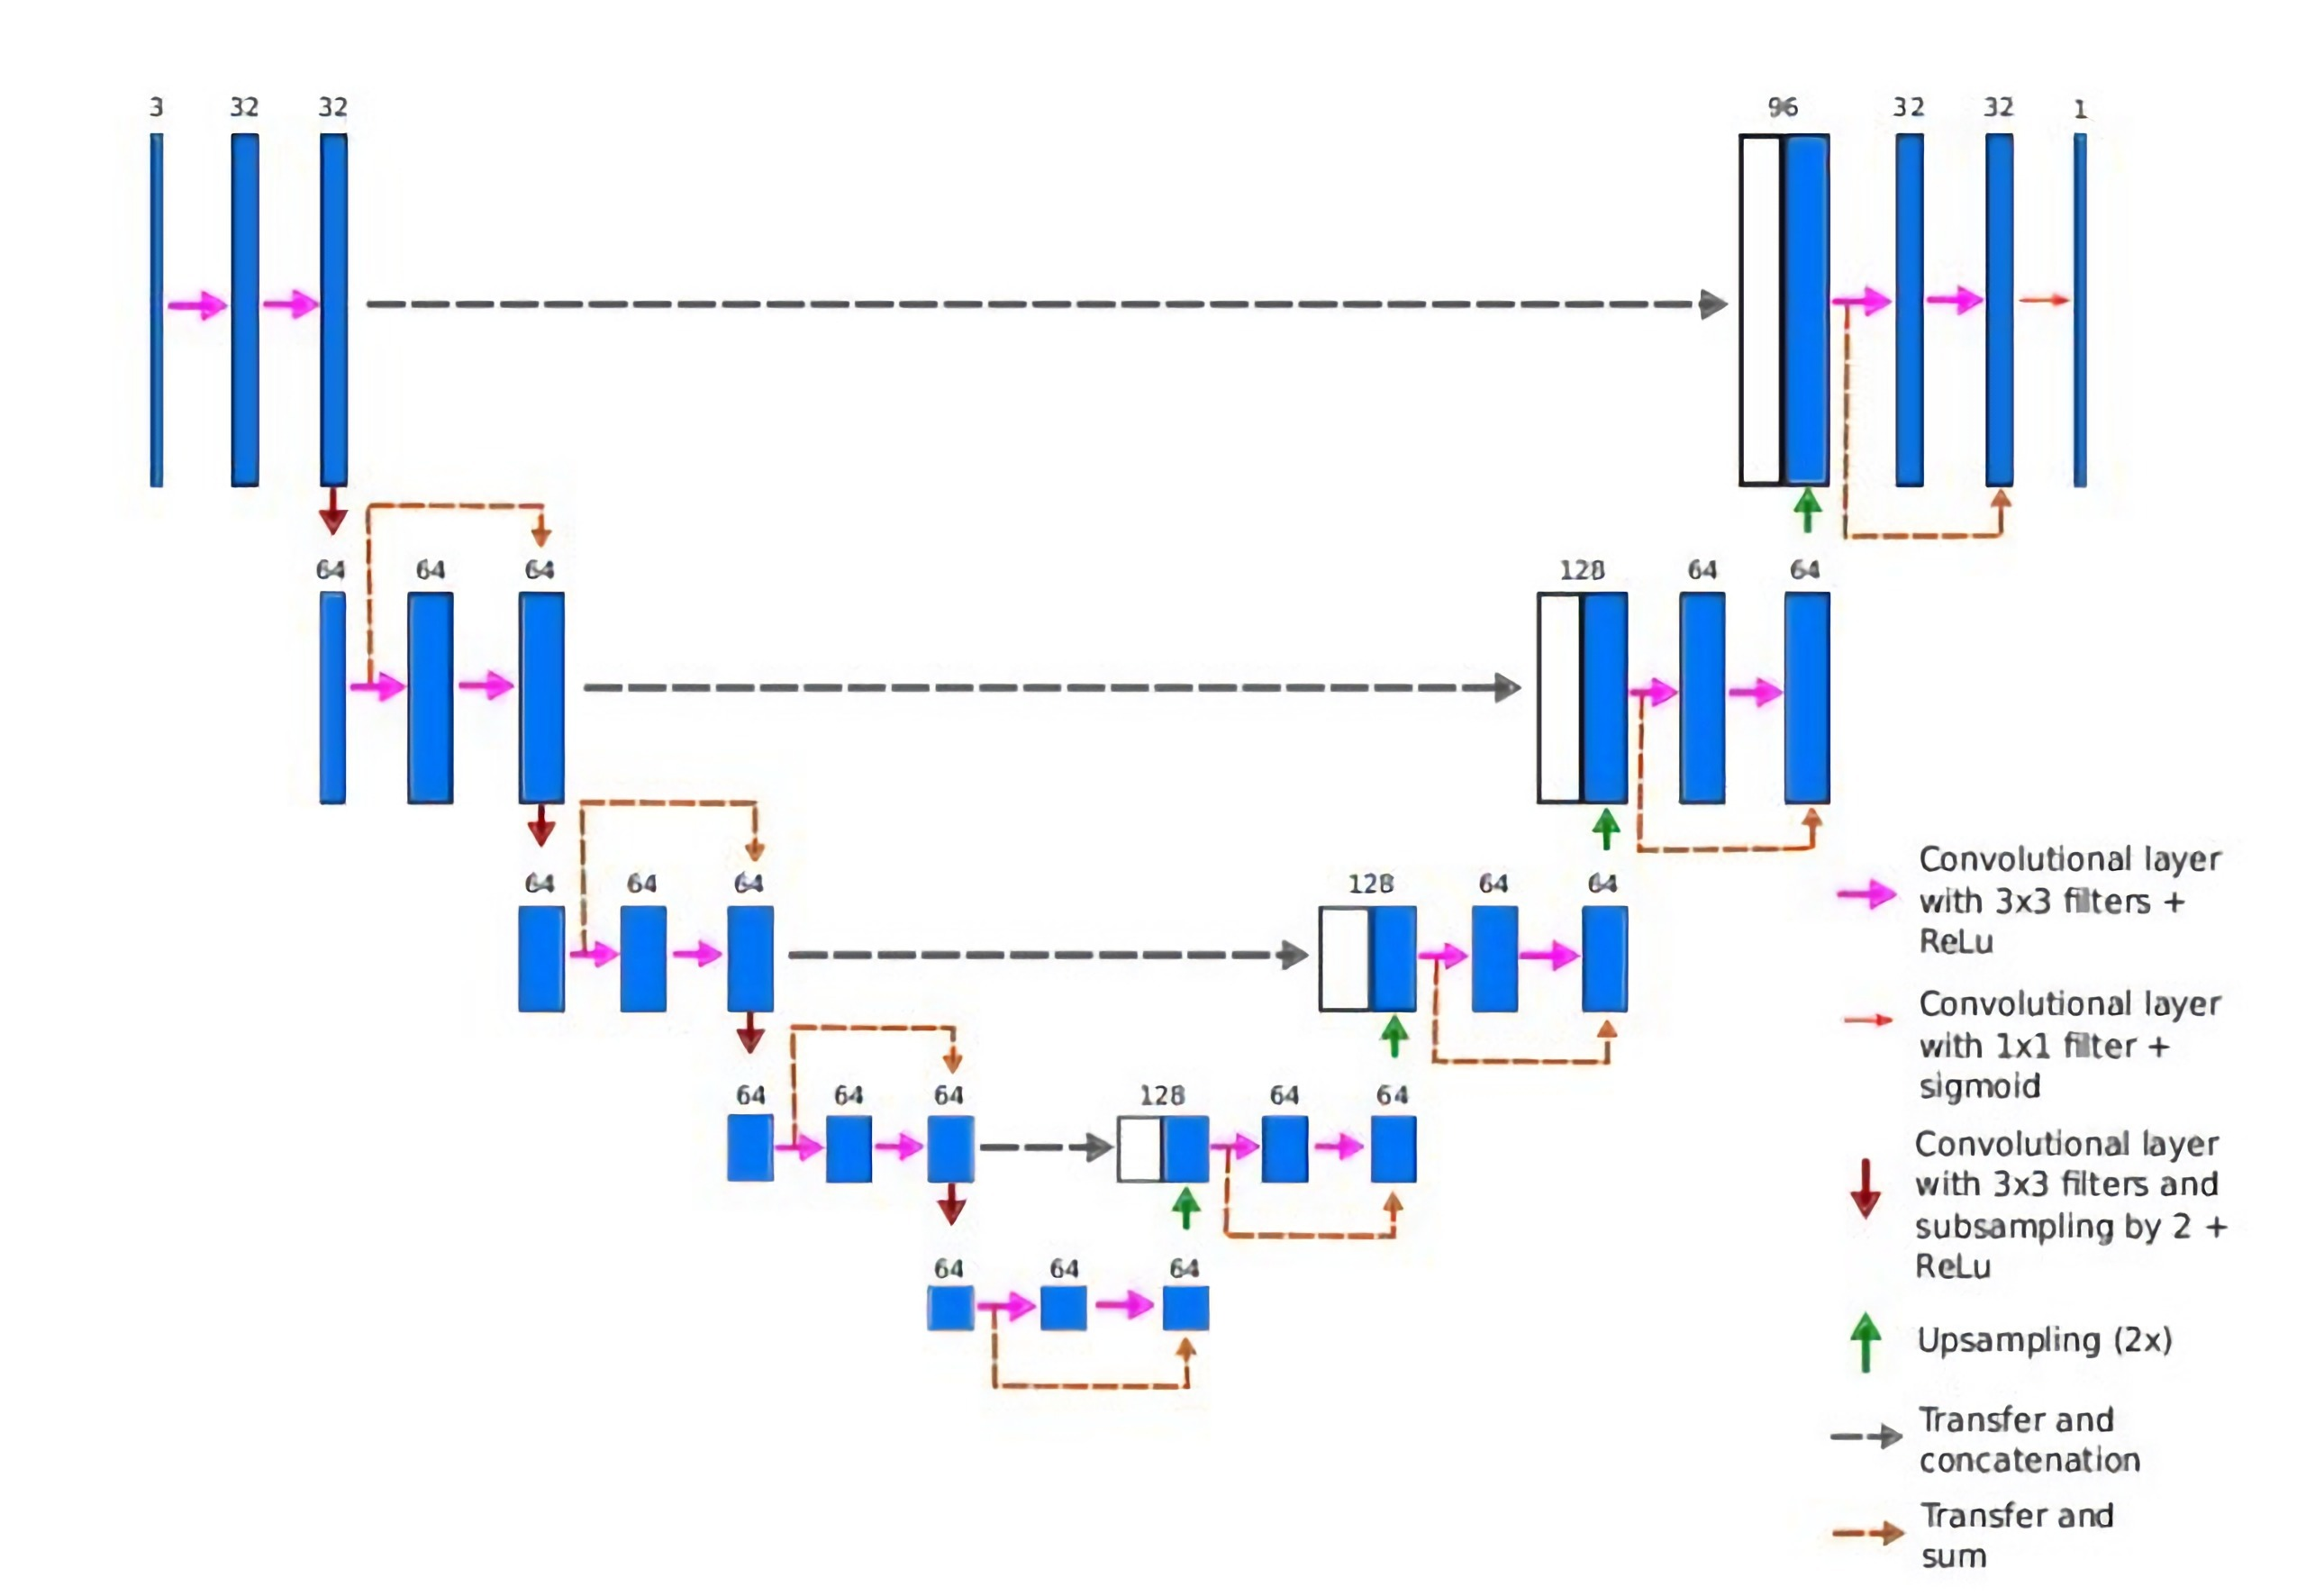
\includegraphics[width=8cm]{Graphics/unet_model.jpg}
    \caption{UNET model\cite{Sevastopolsky_2018}.}
  \end{figure}
\end{frame}

\section{Methods}

\begin{frame}{\insertsectionhead}
  \begin{figure}[H]
    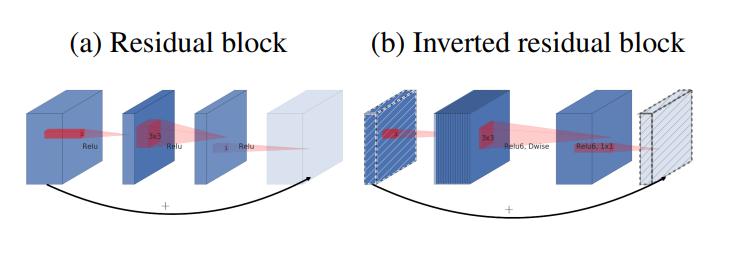
\includegraphics[width=15cm]{Graphics/mobilenetv2.png}
    \caption{MobileNet v2.}
  \end{figure}
\end{frame}

\begin{frame}{\insertsectionhead}
  \begin{figure}[H]
    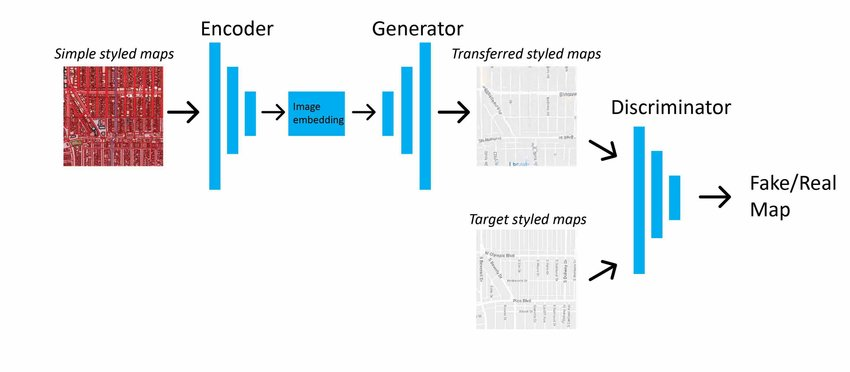
\includegraphics[width=12cm]{Graphics/pix2pix.jpg}
    \caption{pix2pix model.}
  \end{figure}
\end{frame}

\begin{frame}{\insertsectionhead}
  \begin{figure}[H]
    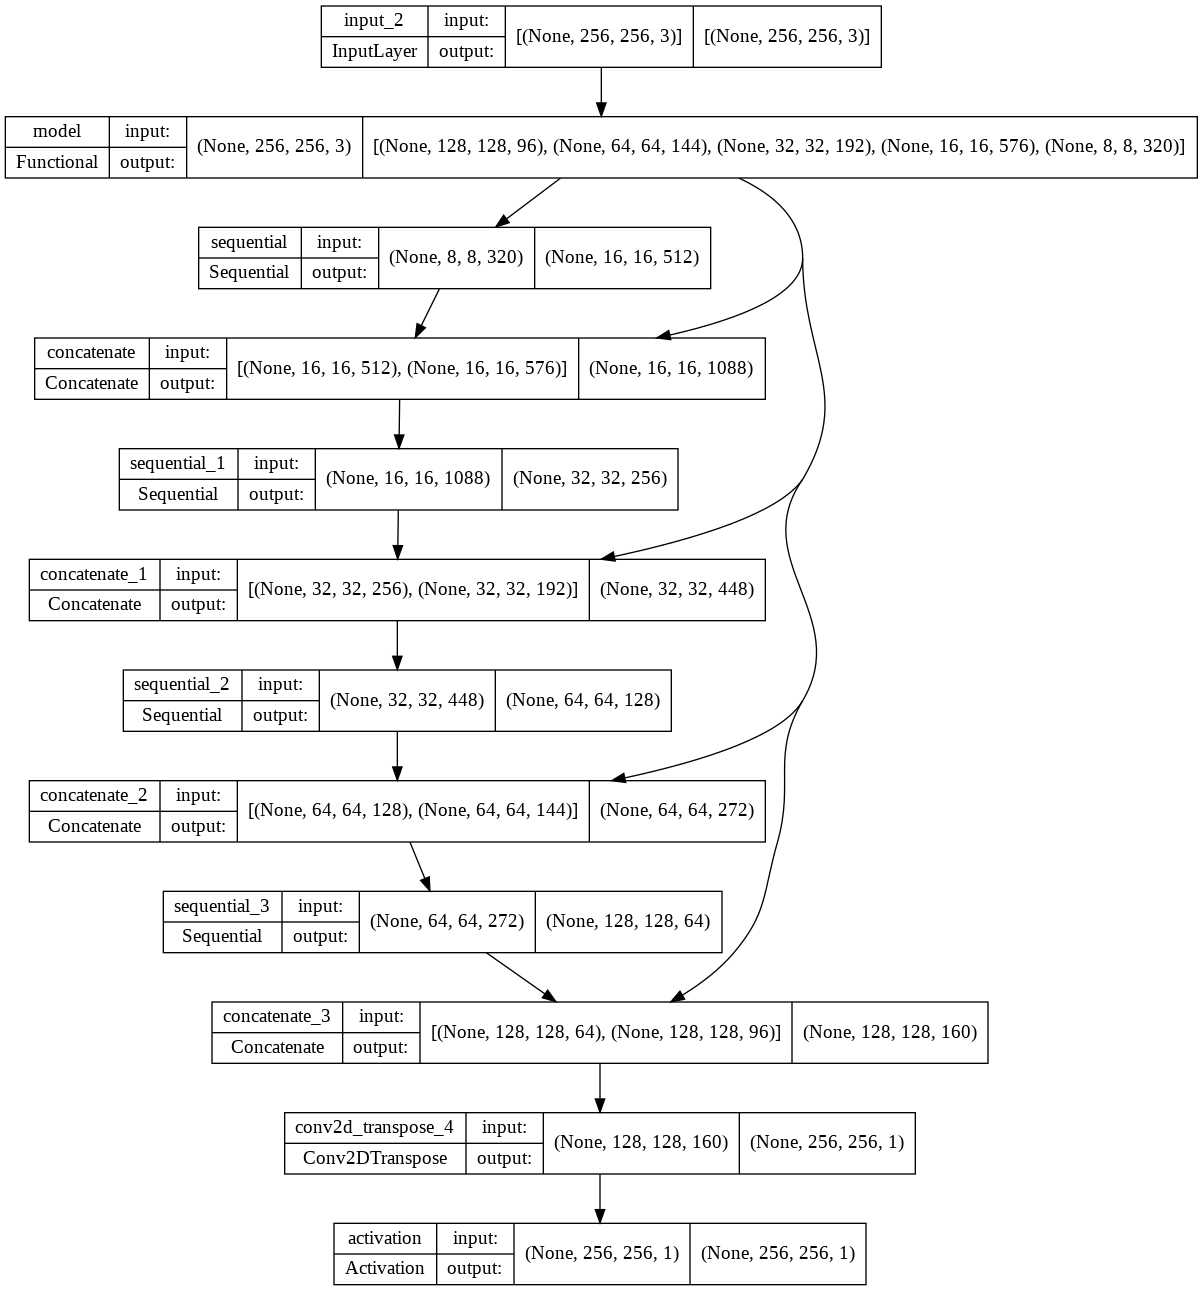
\includegraphics[width=5.5cm]{Graphics/model.png}
    \caption{Model with MobileNetv2 and pix2pix.}
  \end{figure}
\end{frame}

\begin{frame}{\insertsectionhead}
  \begin{figure}[H]
    \begin{subfigure}{5.5cm}
      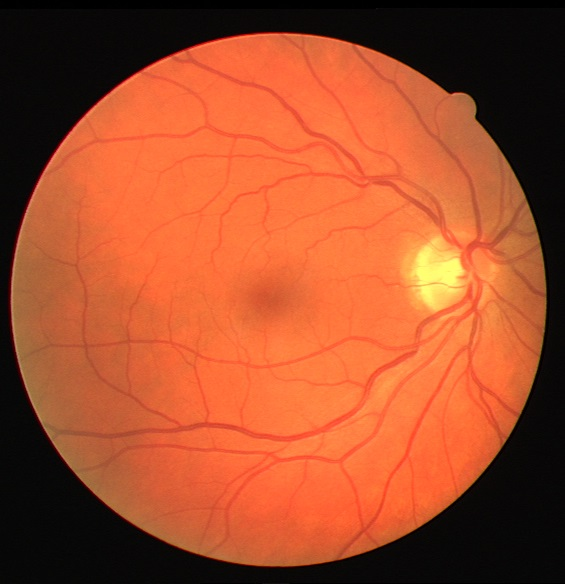
\includegraphics[width=5.5cm]{Graphics/train.jpg}
      \caption{Original image}
    \end{subfigure}
    \hspace*{1cm}
    \begin{subfigure}{5.5cm}
      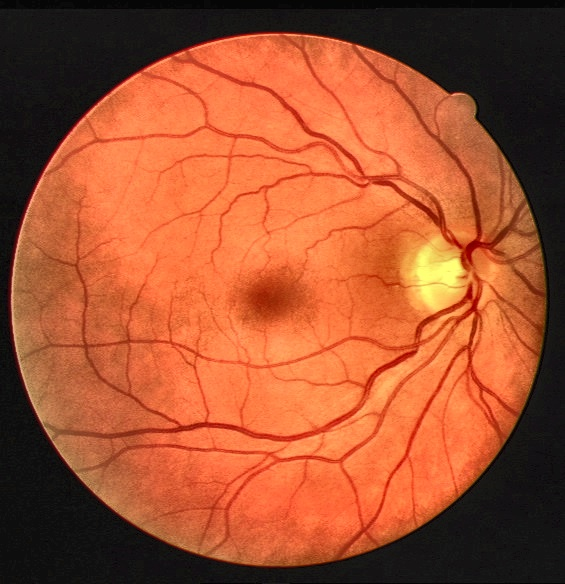
\includegraphics[width=5.5cm]{Graphics/high_contrast.jpg}
      \caption{High contrast image}
    \end{subfigure}
    \caption{Train images.}
  \end{figure}
\end{frame}

\begin{frame}{\insertsectionhead}
  \begin{figure}[H]
    \begin{subfigure}{5.5cm}
      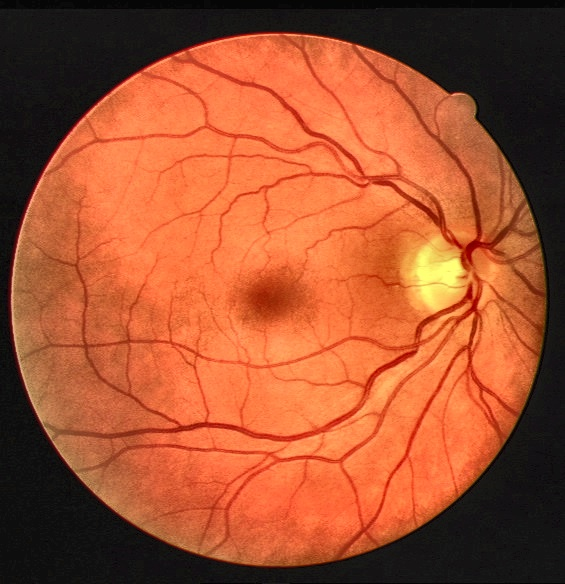
\includegraphics[width=5.5cm]{Graphics/high_contrast.jpg}
      \caption{High contrast image}
    \end{subfigure}
    \begin{subfigure}{1cm}
      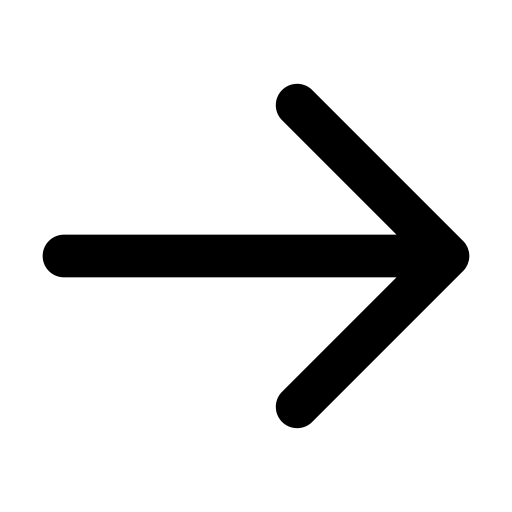
\includegraphics[width=1cm]{Graphics/rightarrow.png}
    \end{subfigure}
    \begin{subfigure}{5.5cm}
      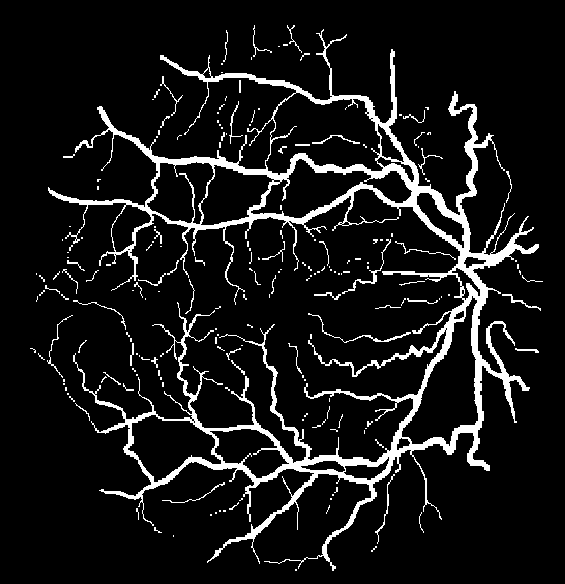
\includegraphics[width=5.5cm]{Graphics/mask.png}
      \caption{Capillary vessels}
    \end{subfigure}
    \caption{Input and output model.}
  \end{figure}
\end{frame}

\section{Results}

\begin{frame}
  \begin{figure}[H]
    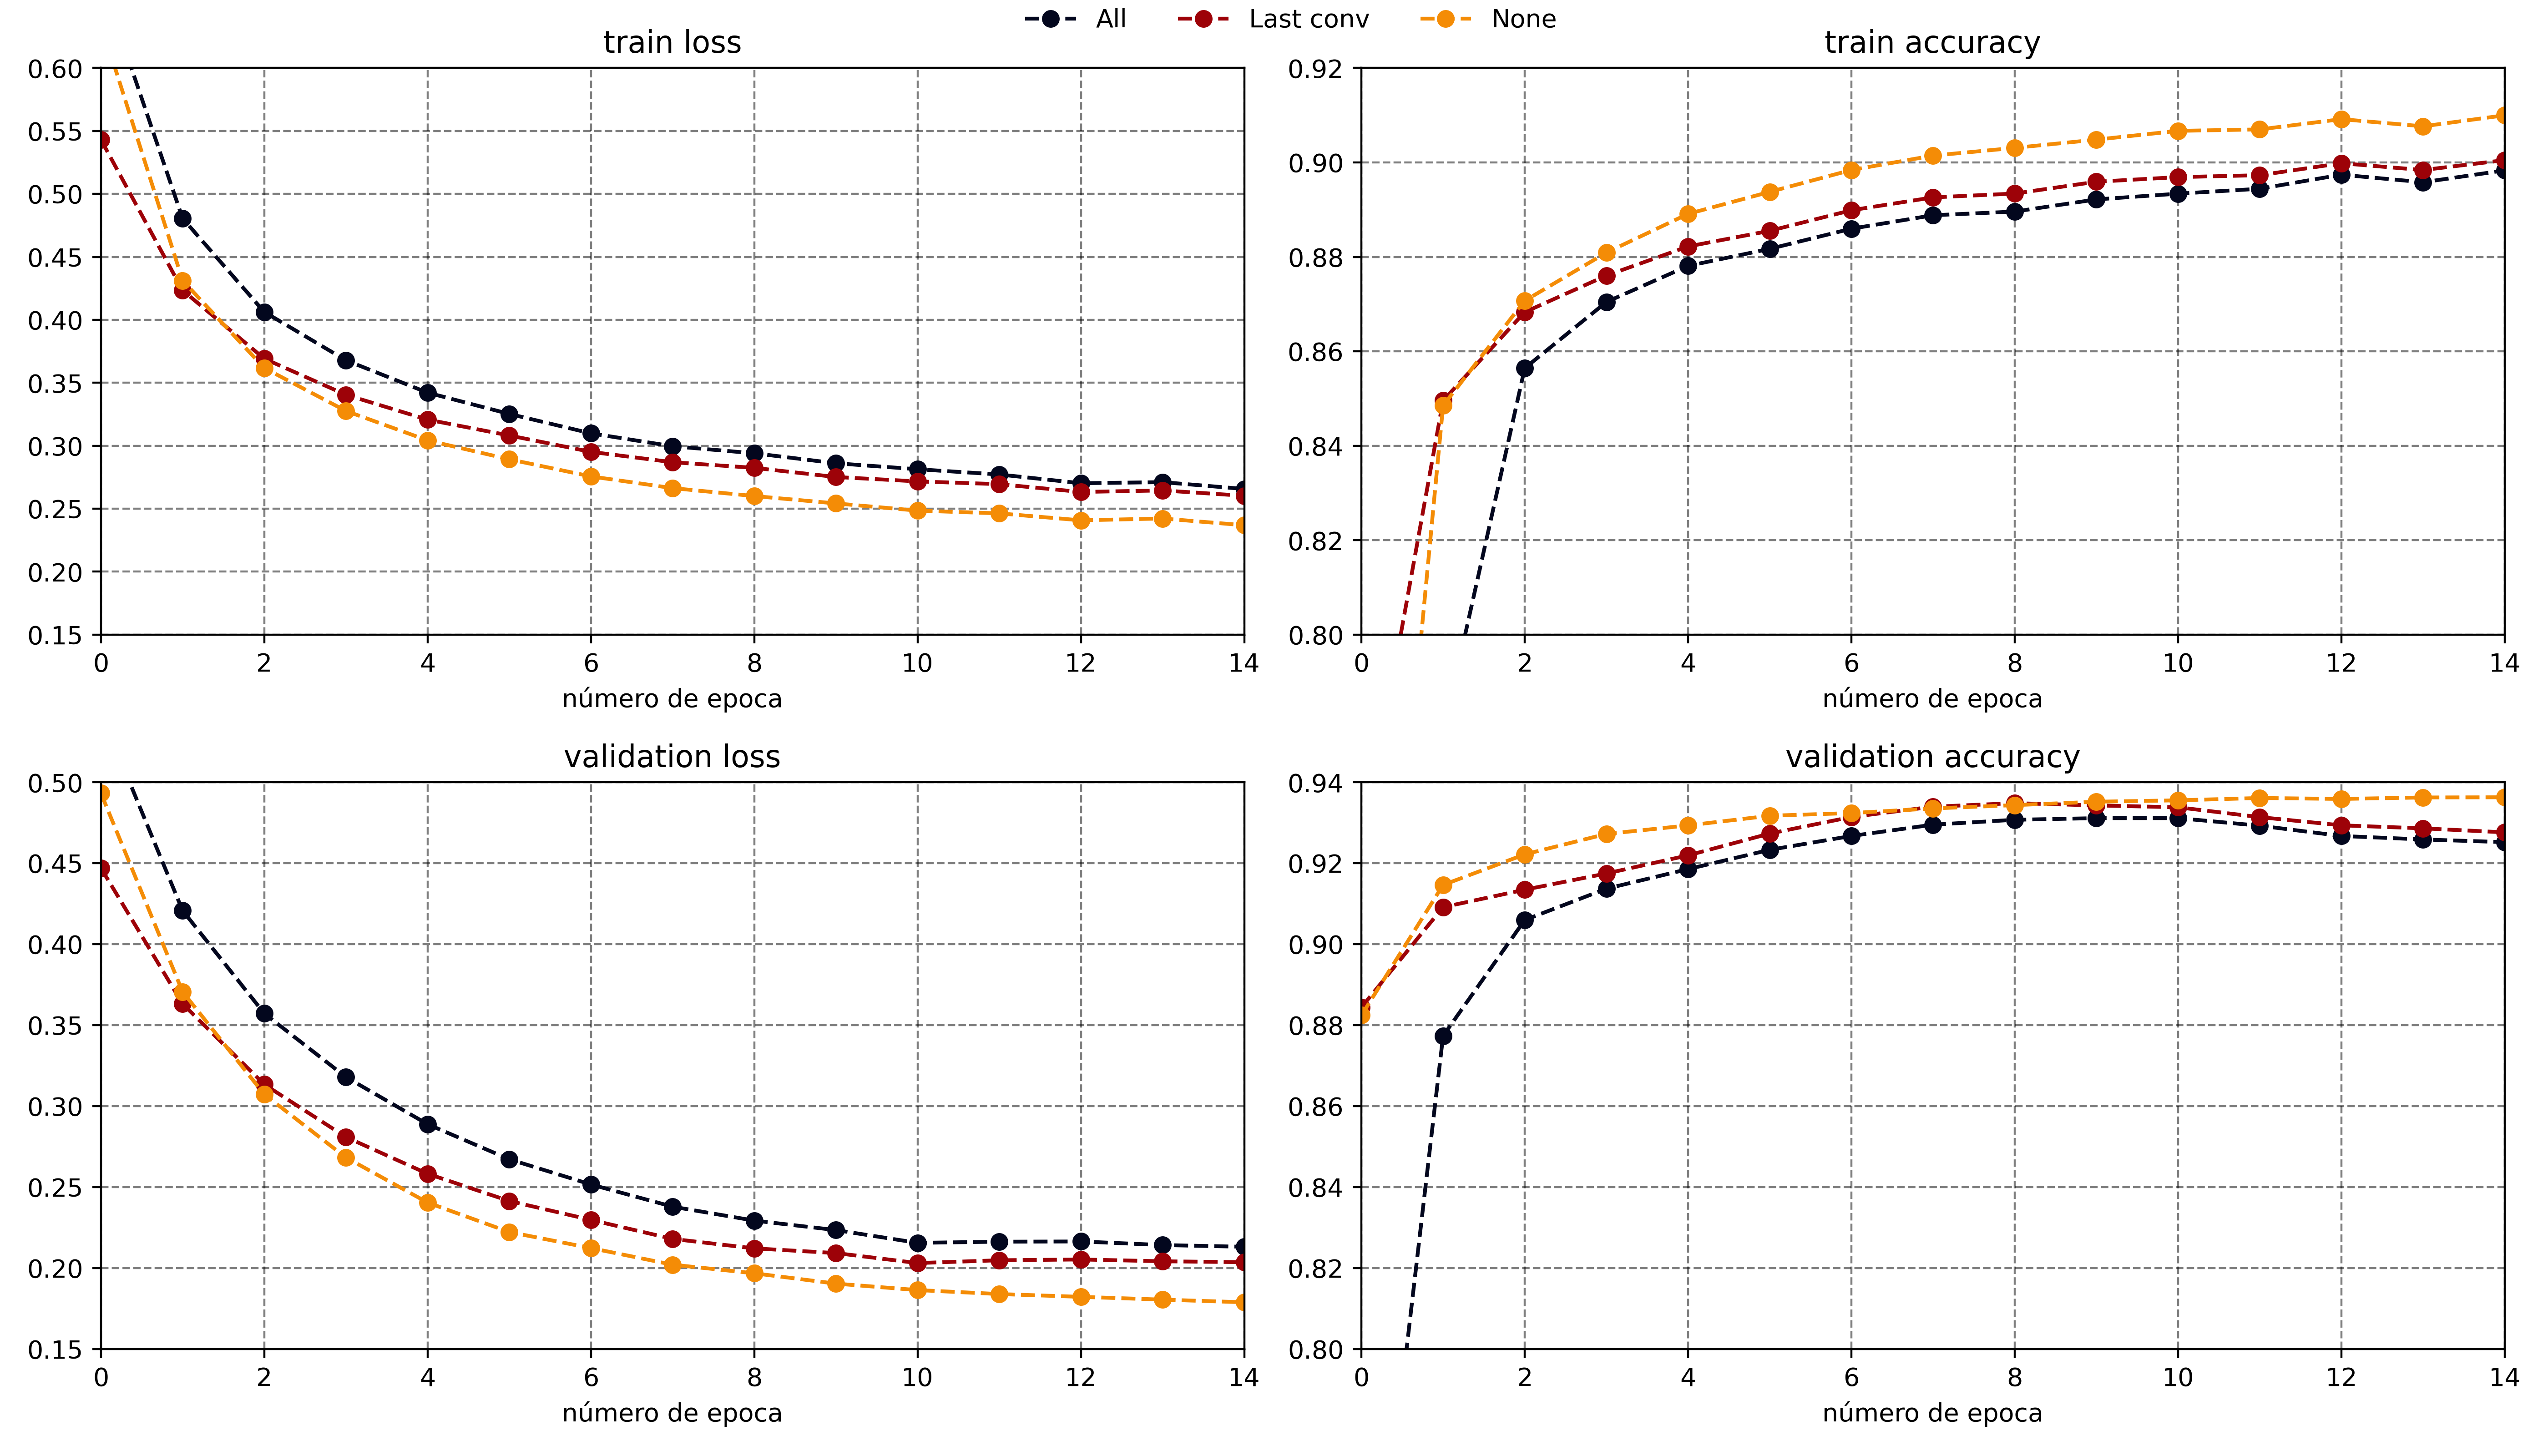
\includegraphics[width=14cm]{Graphics/normal_history.png}
    \caption{History from original images as input model.}
  \end{figure}
\end{frame}

\begin{frame}
  \begin{figure}[H]
    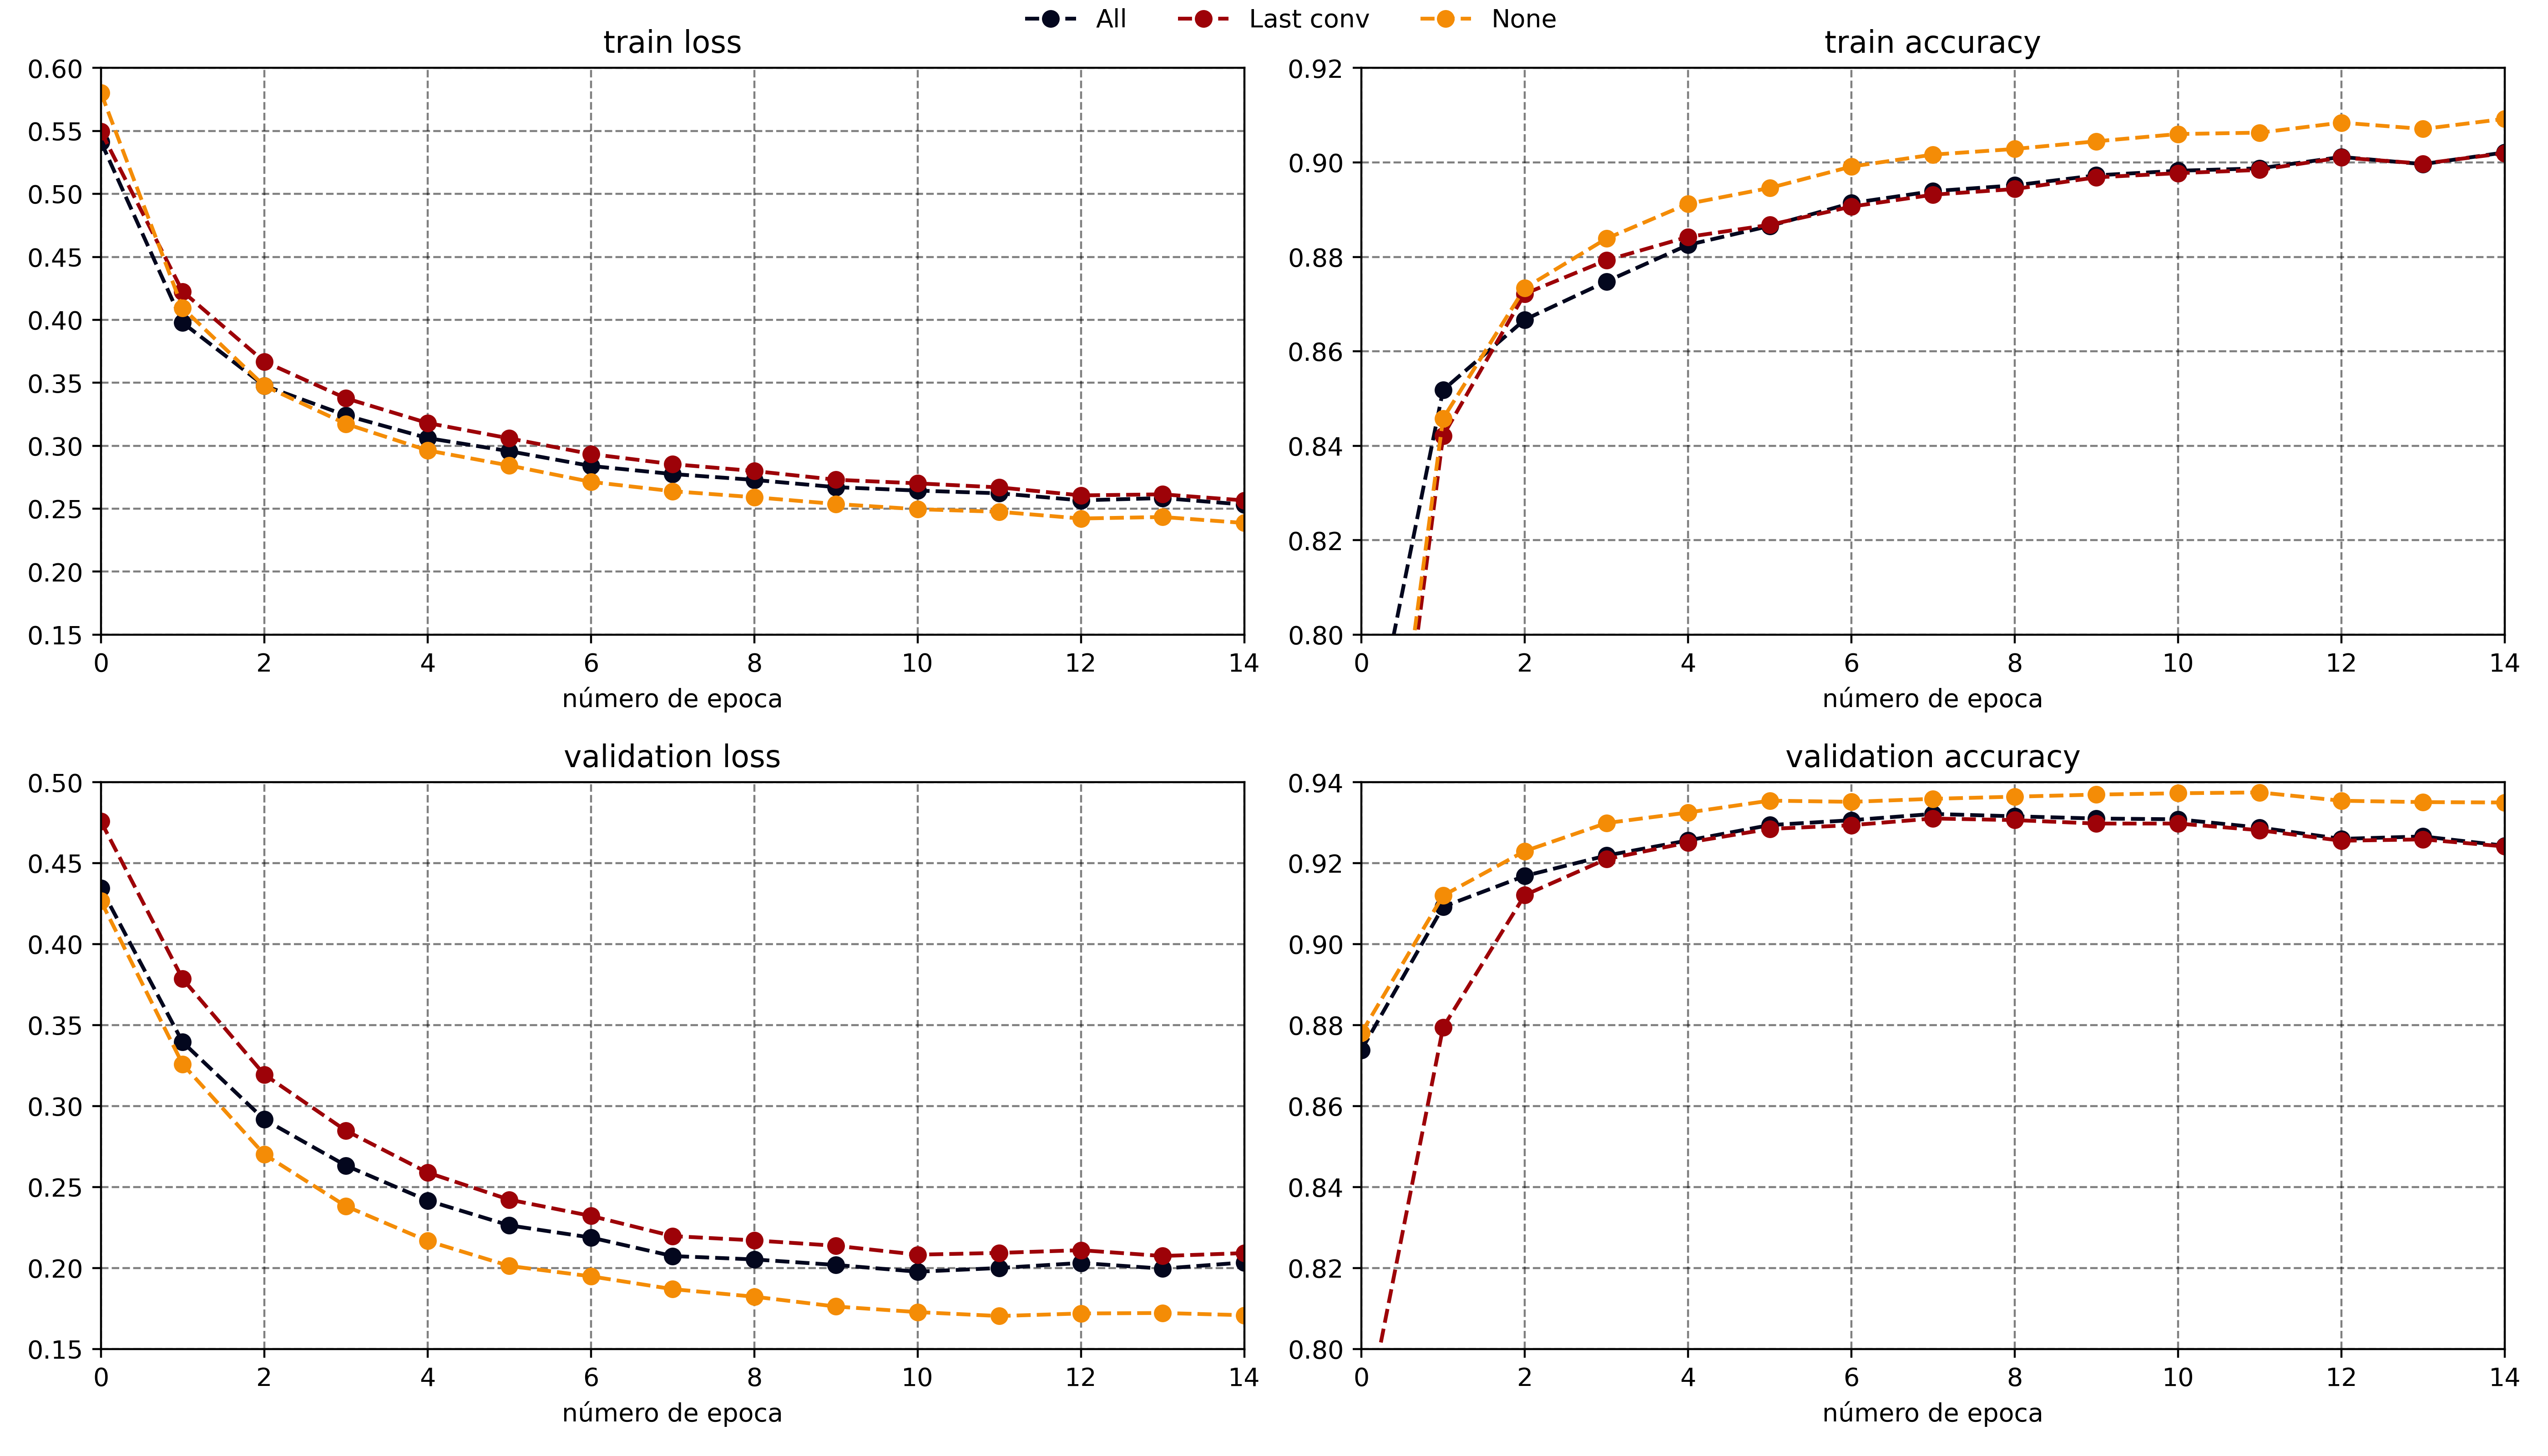
\includegraphics[width=14cm]{Graphics/high_contrast/history.png}
    \caption{History from high contrast images as input model.}
  \end{figure}
\end{frame}

\begin{frame}
  \begin{figure}[H]
    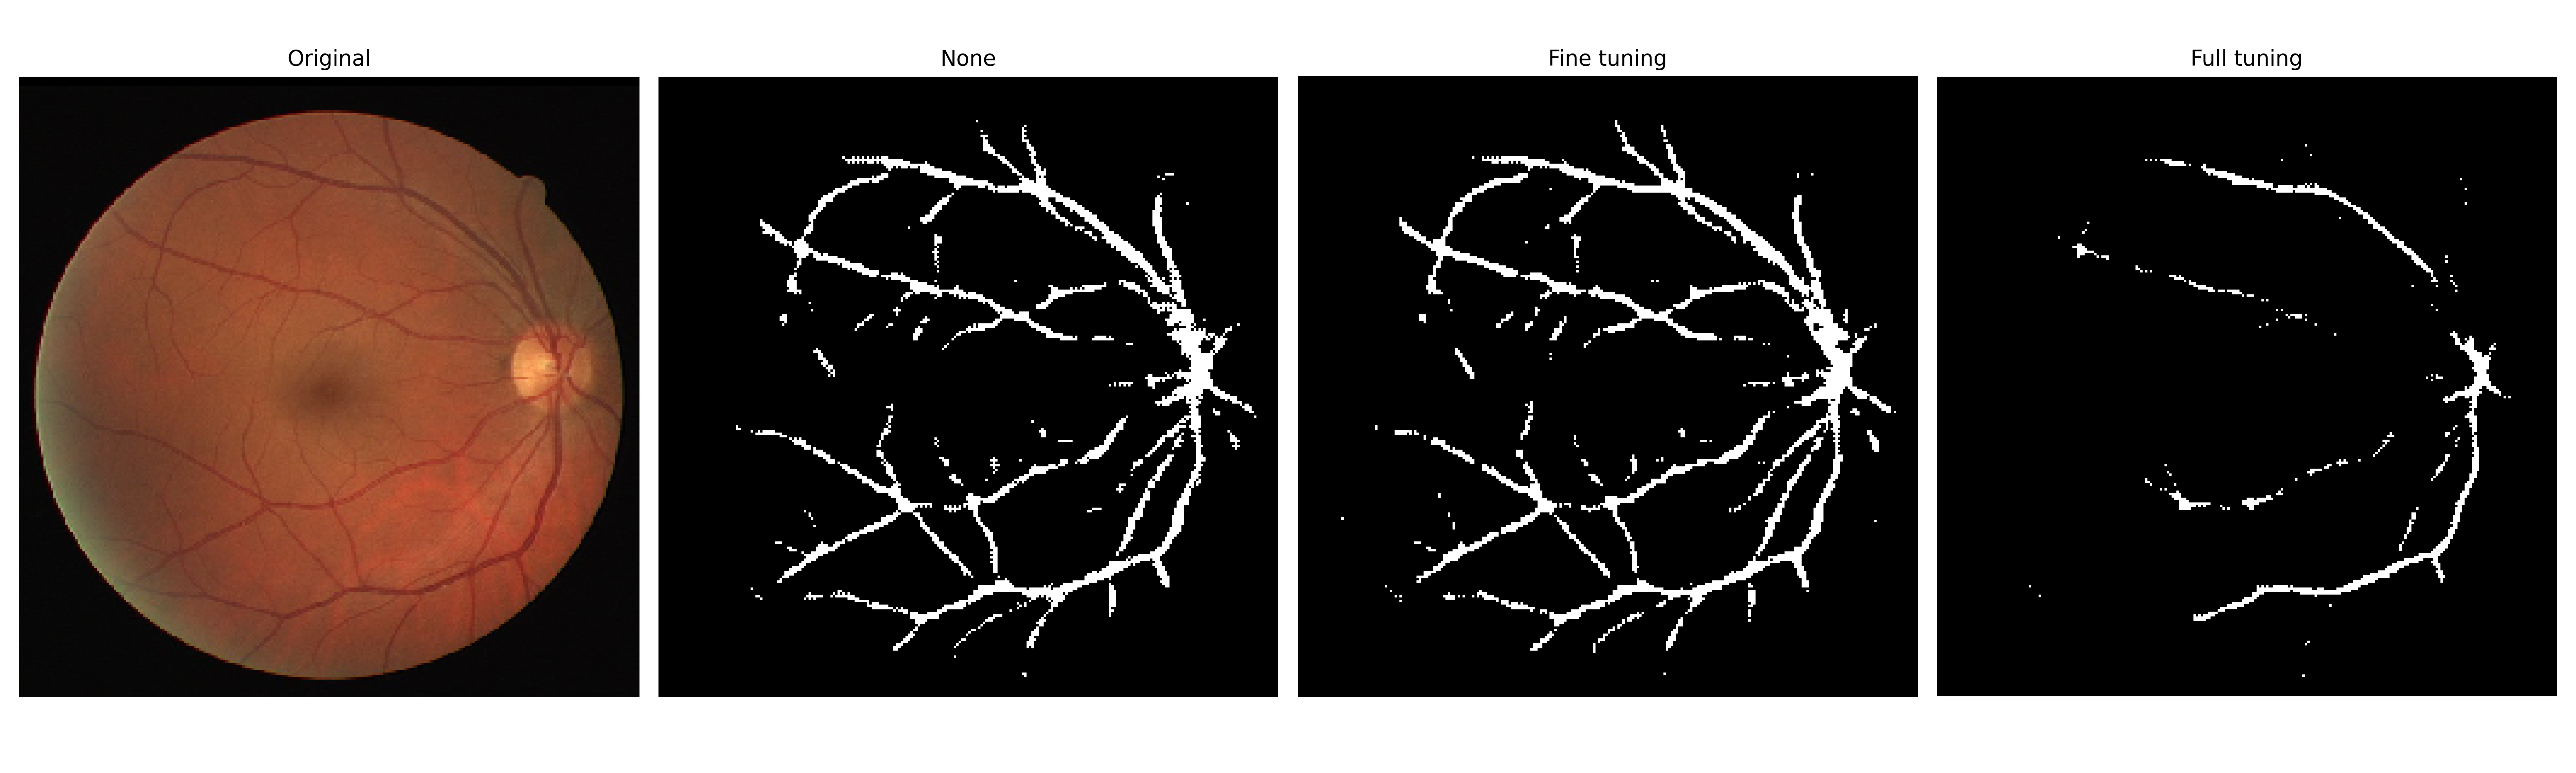
\includegraphics[width=13cm]{Graphics/normal/04.png}
    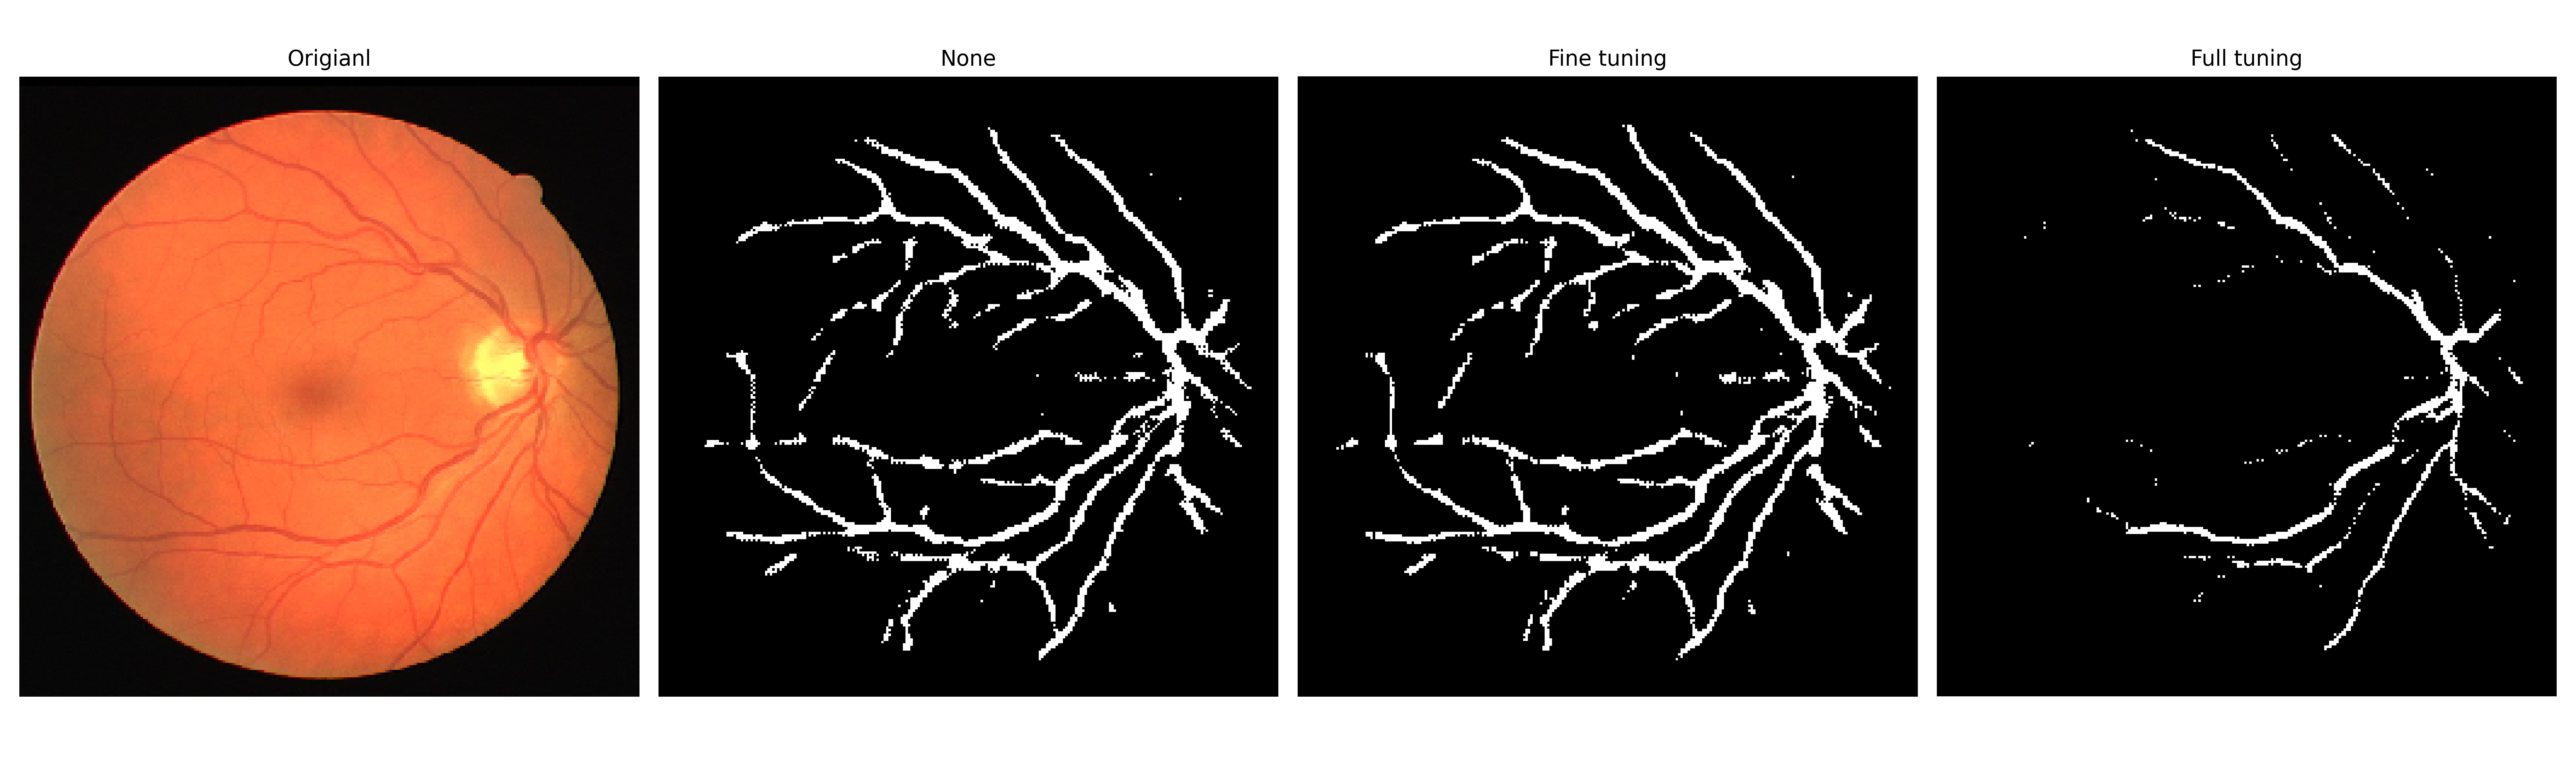
\includegraphics[width=13cm]{Graphics/normal/14.png}
    \caption{Results from original images as input model.}
  \end{figure}
\end{frame}

\begin{frame}
  \begin{figure}[H]
    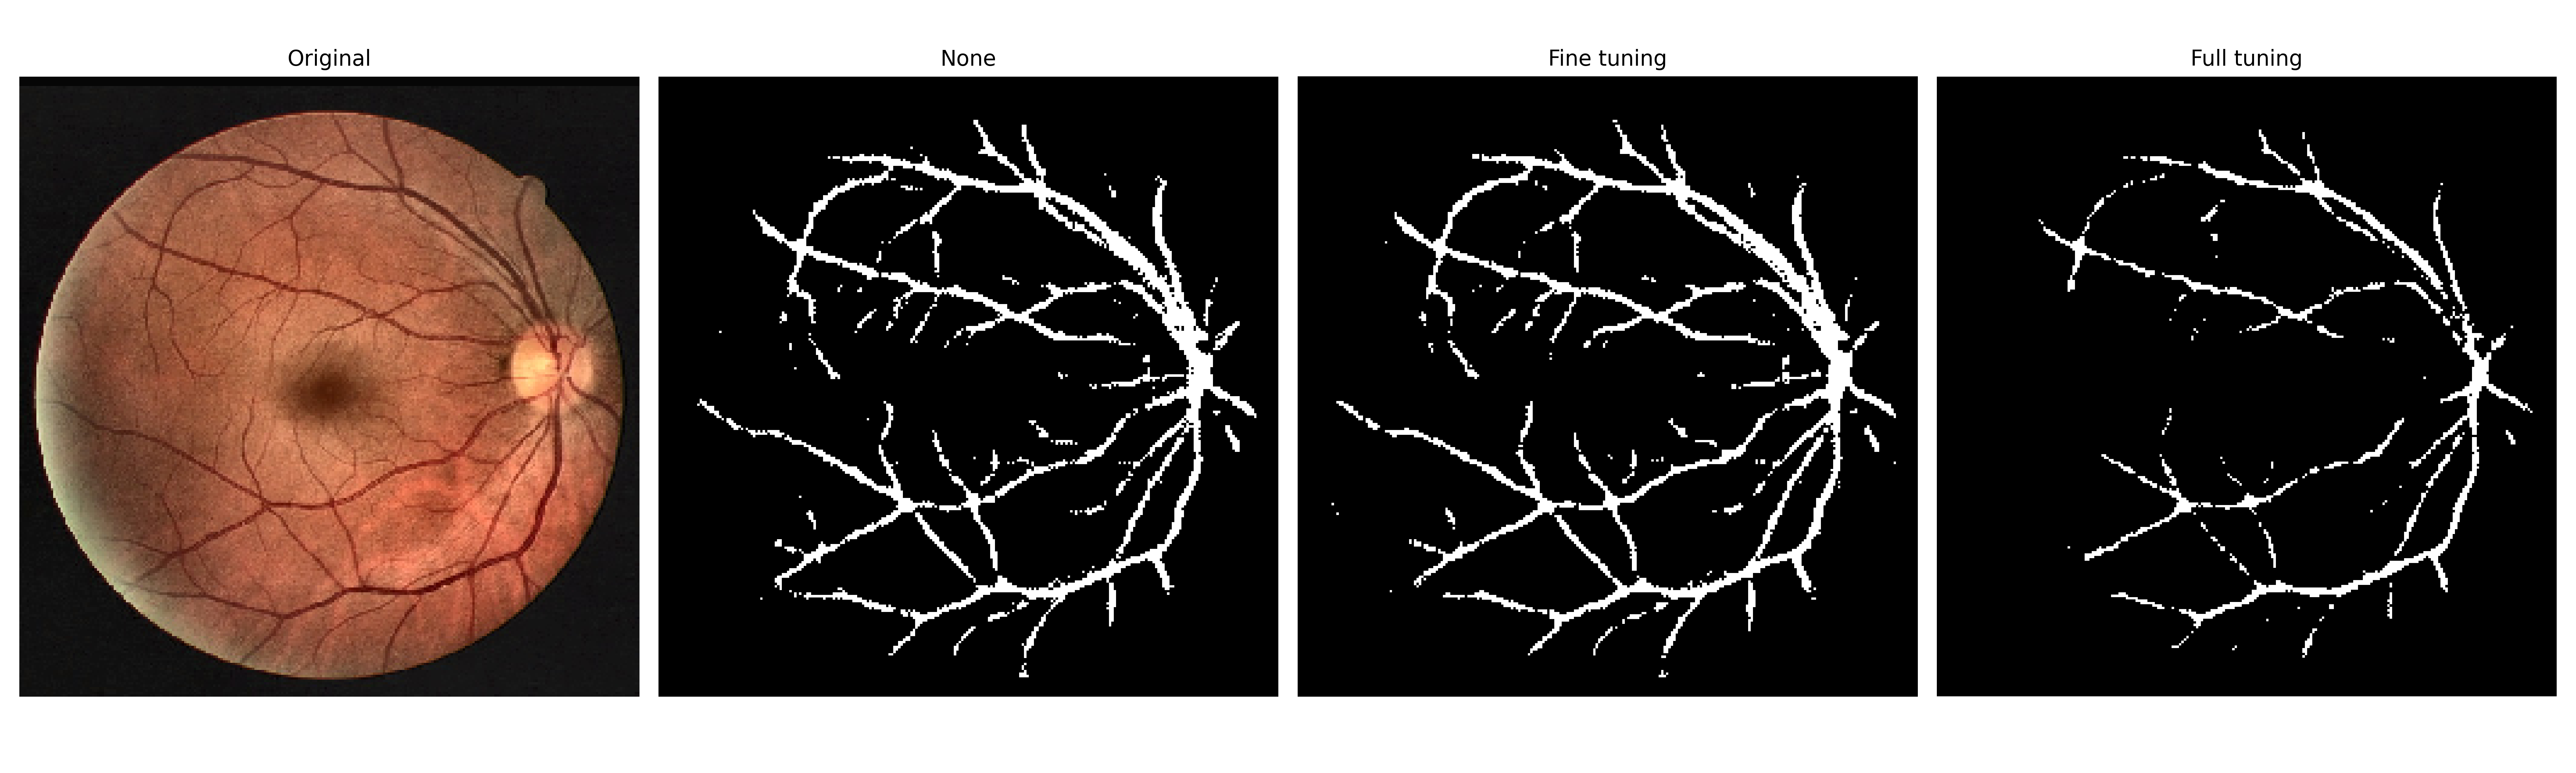
\includegraphics[width=13cm]{Graphics/high_contrast/04.png}
    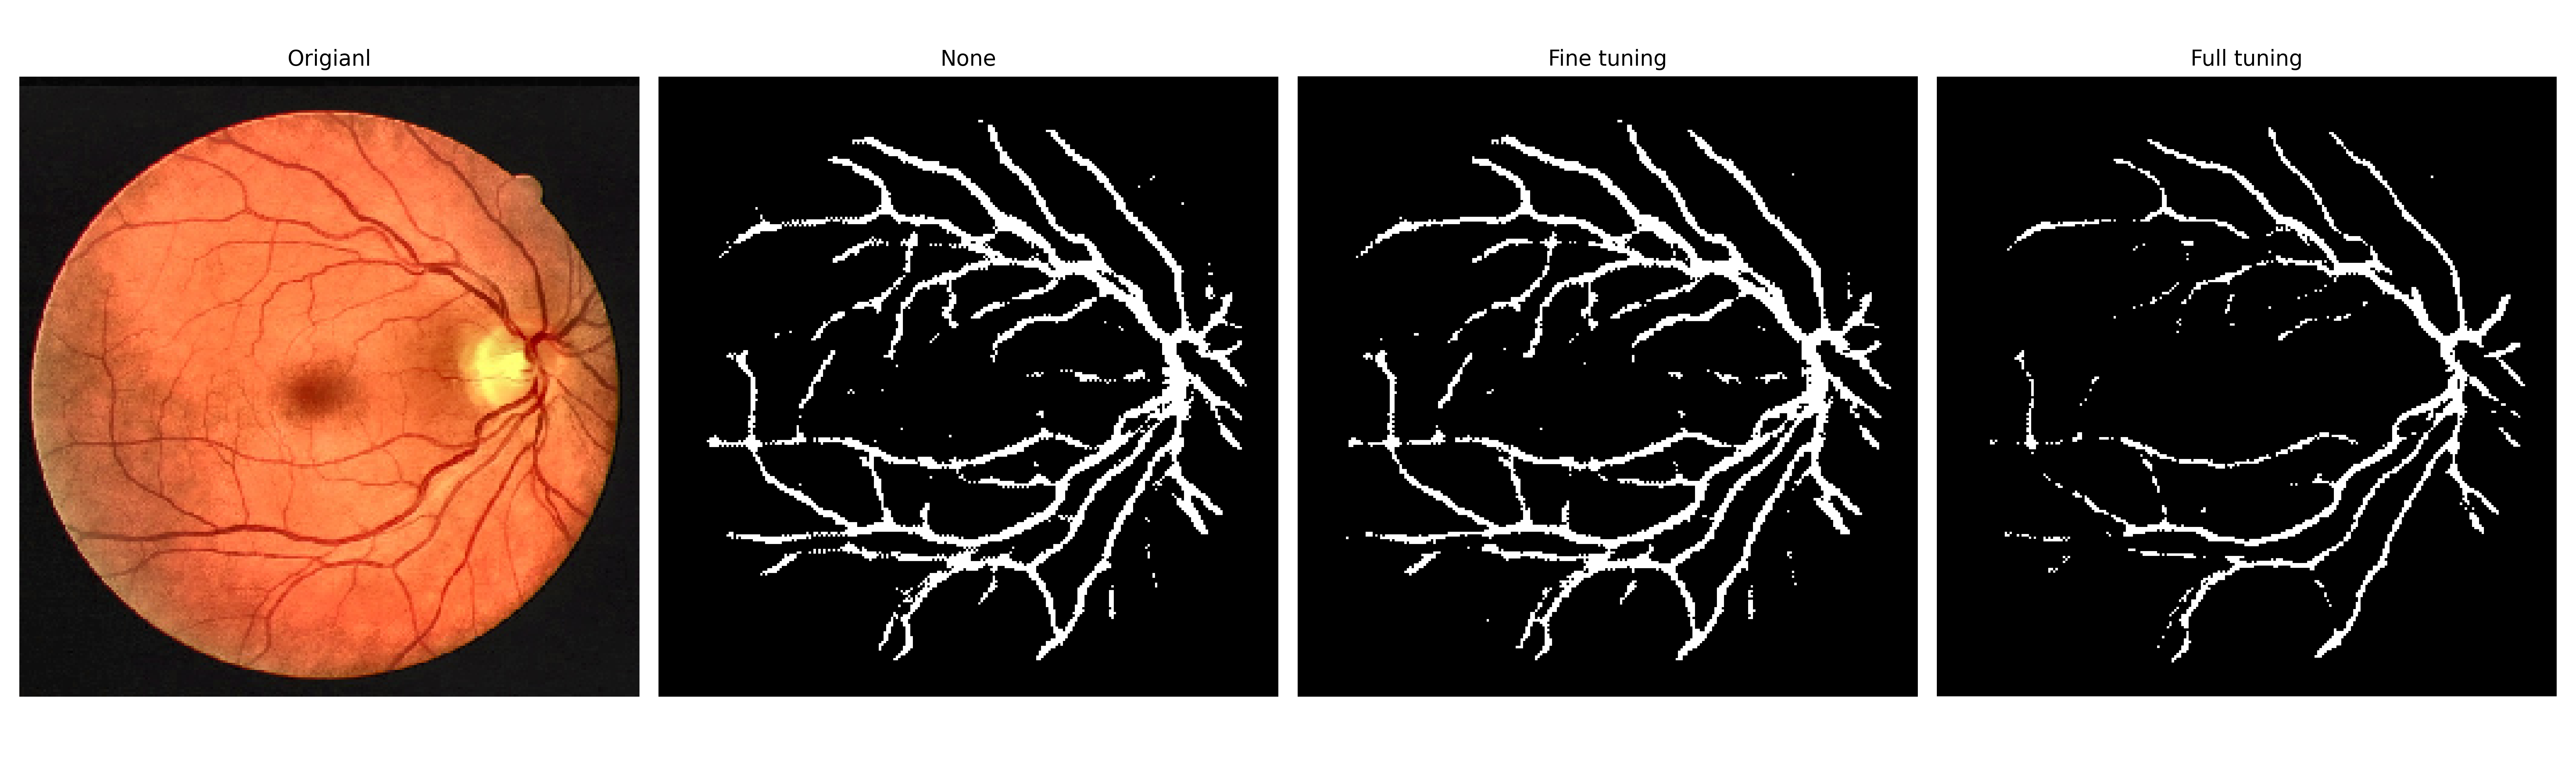
\includegraphics[width=13cm]{Graphics/high_contrast/14.png}
    \caption{Results from high contrast images as input model.}
  \end{figure}
\end{frame}

\section{Conclusions}

\begin{frame}
  \vspace{1cm}
  \begin{minipage}{7cm}
    \begin{figure}[H]
      
\includegraphics[width=7cm]{Graphics/qr-code.png}
    \end{figure}
  \end{minipage}
  \begin{minipage}{7cm}
    \begin{figure}[H]
      
\includegraphics[width=2cm]{Graphics/github.png}\\
      \caption*{\url{https://github.com/giovannilopez9808/Reconocimiento_de_patrones_proyecto_02/}}
    \end{figure}
  \end{minipage}
\end{frame}

\begin{frame}[allowframebreaks]{References}
  \bibliography{references}
  \nocite{*}
  \bibliographystyle{vancouver}
\end{frame}
